\section{実験}
\label{sec:exp}
提案手法をマルウェアに適用して実験を行った.本章では,この実験の目的,方法,結果について解説する.また,結果に対する考察も述べる.
\subsection{実験の目的}
本研究の提案手法により得たマルウェアの実行ログから,マルウェアの挙動を明らかにできていることを示す.

\subsection{実験方法}
今回,11 個の検体を用いた実験と,SMS を送るマルウェア (1 つのマルウェア)を用いた実験の 2 種類の実験を行った.実験の説明の前に \ref{expmalware} で,実験に用いたマルウェアがどのような挙動を示すかを示す.それぞれの実験については, \ref{exp1} , \ref{exp2} で詳しく説明する.

\subsubsection{実験に用いたマルウェア}
\label{expmalware}
今回の実験に用いたマルウェアの挙動を以下に示す \cite{golddream} \cite{basebridge} \cite{droiddreamlight} \cite{crazyapp} \cite{icalendar} \cite{snake} \cite{trojan} .

\begin{enumerate}
\item GoldDream
	\begin{itemize}
	\item	receiver を使うことで,SMS,電話等のシステムイベントをバックグラウンドで監視し,送信元のアドレス,電話,SMS のタイムスタンプ,電話番号をファイルに保存した後,外部のサーバへそのファイルを送信する.
	\item 外部のサーバから 4 種類のコマンドを受け取り,それを実行する.
	\begin{enumerate}
		\item SMS をバックグラウンドで送信する
		\item 電話を発信する
		\item アプリをインストールまたはアンインストールする
		\item ファイルを外部のサーバへアップロードする
	\end{enumerate}
	\end{itemize}

\item basebridge
	\begin{itemize}
	\item アプリのアップグレードを促すダイアログを出し.そこでアップグレードを選択すると,basebridge は com.android.battery を感染した端末にインストールする.
	\item 外部のサーバとの通信を行い,番号などが載った configuration list  をダウンロードし,この情報を基に,SMS を送信する.
	\item SMS をバックグラウンドで送信したことをユーザに気付かれないようにするために,モバイルキャリアからの課金確認の SMS をブロックする.
	\end{itemize}

\item com.tencent.qqgame
	\begin{itemize}
	\item 挙動は GoldDream と同じ
	\end{itemize}

\item Beauty Breast
	\begin{itemize}
	\item 感染した端末に電話がかかってくると,その端末の端末番号,機種名,SDK バージョン等の端末の情報を外部サーバへ送る.
	\item 新しいパッケージのインストールと,それを促すプロンプトを表示する.
	\item マルウェア自身では,上の挙動をすることはなく,ユーザの何らかの操作無しでは実行されない.
	\end{itemize}

\item Beauty Leg
	\begin{itemize}
	\item Beauty Breast と挙動は同じ
	\end{itemize}

\item Beauty Girl
	\begin{itemize}
	\item Beauty Breast と挙動は同じ
	\end{itemize}

\item crazy app
	\begin{itemize}
	\item 感染した端末の IMEI (端末を識別する番号) を外部サーバへ送信する.
	\item  ブラウザのブックマーク情報とブラウザの閲覧履歴をアップロードする.
	\end{itemize}
\item iCalendar
	\begin{itemize}
	\item 有料サービスに登録させるためにある番号へ SMS をバックグラウンドで送信する.
	\item SMS  を送信できたかどうかをタグとして内部で記録している.
	\item ユーザに気づかれるのを防ぐために一度しか行われない.
	\end{itemize}
	
\item iMatch
	\begin{itemize}
	\item 挙動は iCalendar と同じだが,SMS は起動する度に何度も送信される.
	\end{itemize}
	
\item Snake App
	\begin{itemize}
	\item バックグラウンドで外部サーバに端末の GPS 情報を送信する.
	\item 表向きはゲームアプリとして振舞っている.
	\end{itemize}
	

\item com.tencent.qq
	\begin{itemize}
	\item 感染した端末の IMEI 番号,電話番号,登録者 ID,SIM カードのシリアル番号を盗み,外部のサーバへ送信する.
	\item 過去に SMS を送った電話番号を収集する.
	\item 外部のサーバからコマンドを受け取り,以下の動作を行う
	\begin{enumerate}
		\item SMS コンテンツや URL をサーバから受け取った電話番号へ送信する.
		\item ある URL から APK ファイルをダウンロードし,それをインストールする.
		\item ブラウザにブックマークを追加する.
		\item ある URL へ誘導するポップアップを表示する.
	\end{enumerate}
	\item ログファイルに記載されている電話番号からの SMS をブロックする.
	\end{itemize}
\end{enumerate}

\subsubsection{実験 1:11 個の検体を用いた実験}
\label{exp1}
実際にマルウェアにログコードを挿入する前の準備として,ログコードを挿入するクラスを絞り込む.なぜこの処理が必要であるかというと,マルウェアのソースコード中の全てのクラスのメソッドにログコードを挿入してしまうと,不必要なログが大量にでてきてしまうためだ.例えば,ゲームアプリの場合,常に描画のためのメソッドが実行されている.このようなメソッドと不正を動きをしているメソッドのログが混ざって出力されてしまうと,解析が非常に行いづらい.マルウェアのソースコード ( Java クラスファイル) を探索し,"install", "download", "SMS", "remote" などのマルウェアの代表的な挙動を表す単語を含むメソッドのクラスを不正な動きをするクラスとみなし,コードを挿入するクラスとする.

コードを挿入するクラスを決定したらそれぞれのマルウェアのメソッドの先頭にログコードを挿入した.ログコードが挿入されたマルウェアを Nexus 5 (Android 4.4.4) にインストールした後,手動でマルウェアを起動した.

\subsubsection{実験 2:SMS  を送るマルウェアの実験}
\label{exp2}
実験 2 では,SMS を送るマルウェアである iMatch に対してのみ行った.実験 1 と同様にコードを挿入するクラスを決定した後に,そのクラスのメソッドに対して,メソッド呼び出しの前後にログコードを挿入した.その後,メソッドの先頭へログコードを挿入する.(これは実験 1 と同じ操作)そして,ログコードを挿入した iMatch を Nexus 5 (Android 4.4.4) にインストールして,これを起動した.

\subsection{実験結果}
\subsubsection{実験 1 の結果}
11 個中,8 個のマルウェアからログを得ることができた.その 8 個の中の 5 個では,不正な動きを示すログを得ることができた.これら 5 つの結果を以下に示す.
GoldDream
\begin{figure}[t]
\begin{center}
\graphicspath{{./epsfiles/}}
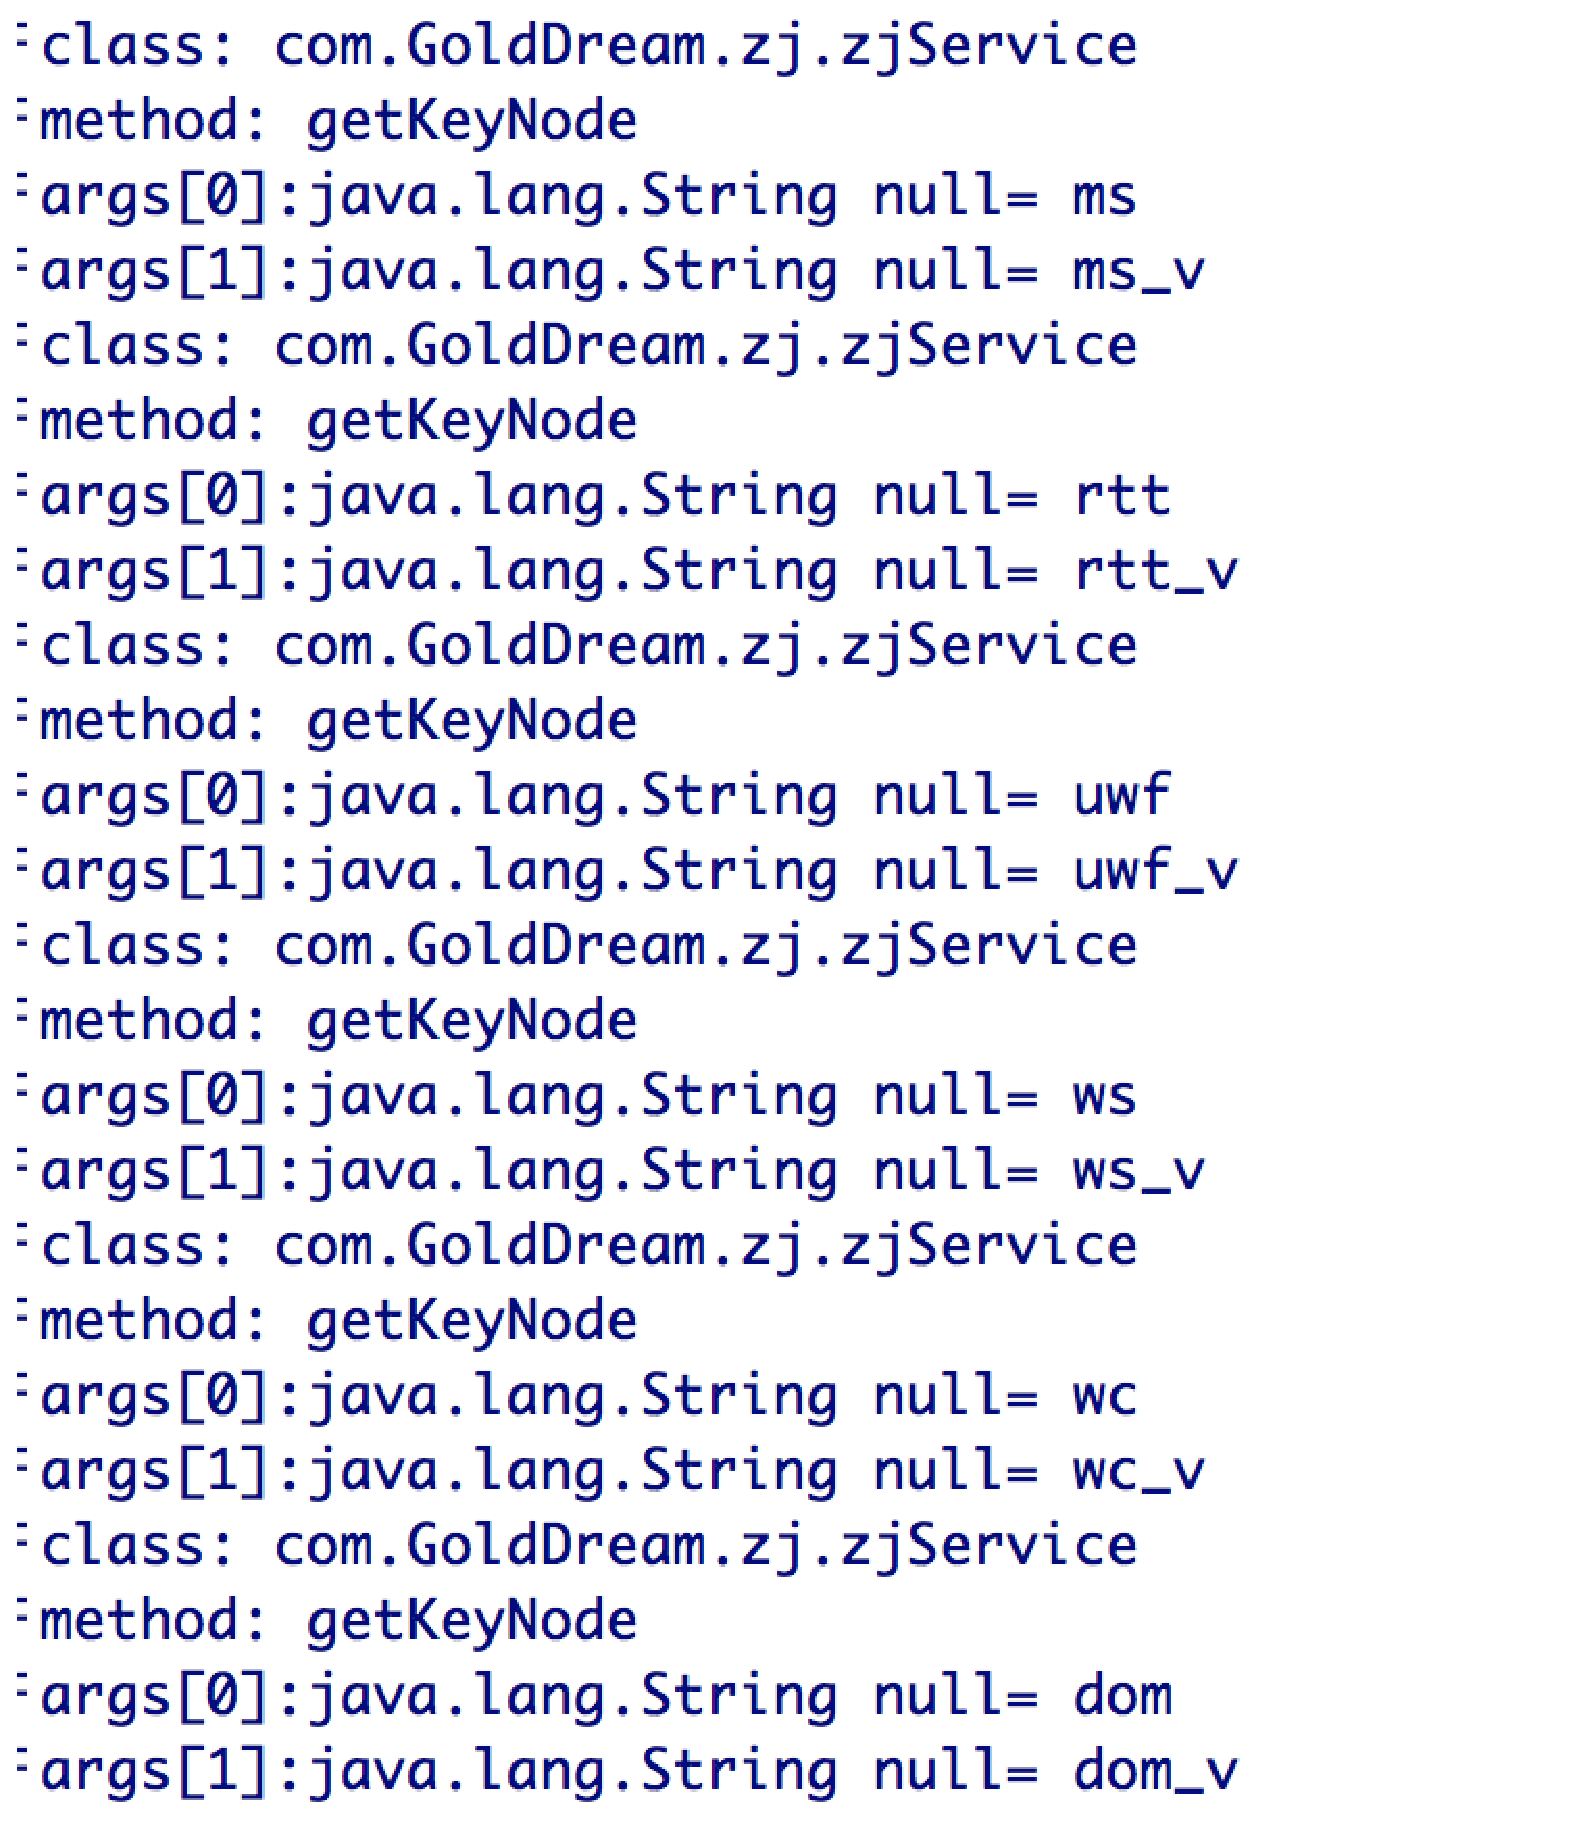
\includegraphics[scale=0.4]{getkeynodezjservice.eps}
\end{center}
\caption{getKeyNode}
\label{zjservicegetkey}
\end{figure}

com.tecent.qqgame

iCalendar

iMatch

com.tencent.qq

3 個のマルウェアからは,ログを得ることはできたが,メソッド名が意味を為しておらず,挙動を特定することができなかった.
beauty leg, breast, girl の 3 つ

ログが出なかったもの

\subsubsection{実験 2 の結果}

